%%%%%%%%%%%%%%%%%%%%%%%%%%%%%%%%%%%%%%%%%%%%%%%%%%%%%%%%%%%%%%%%%%%%%%%%%%%%%%%%
%2345678901234567890123456789012345678901234567890123456789012345678901234567890
%        1         2         3         4         5         6         7         8

%\documentclass[letterpaper, 10 pt, conference]{ieeeconf}  % Comment this line out
                                                          % if you need a4paper
\documentclass[a4paper, 11pt]{report}      % Use this line for a4
                                                          % paper

\usepackage[T1]{fontenc}
\usepackage{csquotes}
\usepackage{natbib}
\usepackage{graphicx}

%\usepackage{culmus}
%\usepackage{fontspec}
%\usepackage{polyglossia}
%\newfontfamily{\hebrewfont}{David CLM}


%\usepackage[english,hebrew]{babel}

%\selectlanguage{english}
\usepackage{fontspec}
\usepackage{appendix}

\bibliographystyle{abbrvnat}

\setcitestyle{authoryear,round}

\pagestyle{myheadings} 

\renewcommand{\thesection}{\arabic{section}}
%\DeclareUnicodeCharacter{}
% The following packages can be found on http:\\www.ctan.org
%\usepackage{graphics} % for pdf, bitmapped graphics files
%\usepackage{epsfig} % for postscript graphics files
%\usepackage{mathptmx} % assumes new font selection scheme installed
%\usepackage{mathptmx} % assumes new font selection scheme installed
%\usepackage{amsmath} % assumes amsmath package installed
%\usepackage{amssymb}  % assumes amsmath package installed

\begin{document}

\begin{titlepage} % Suppresses headers and footers on the title page
	
	{\centering % Centre everything on the title page
	% \rule{\textwidth}{1pt} % Thick horizontal rule
	
	% \vspace{2pt}\vspace{-\baselineskip} 
	% Whitespace between rules
	
	% \rule{\textwidth}{0.4pt} % Thin horizontal rule
		\vspace{0.05\textheight} % Whitespace between 
	
	%--------------------pastes randomly----------------------------
	%	Top rules
	%------------------------------------------------
	\huge{Department of Computer Science
	
	Bar-Ilan University
	
	\vspace{30pt}}
	\Large{
	M. Sc. Research Proposal - December 2020
	}
	\vspace{15pt}
	
	%\vspace{0.1\textheight} % Whitespace between the top rules and title
	
	%------------------------------------------------
	%	Title
	%------------------------------------------------
{\renewcommand{\baselinestretch}{1.8}\selectfont
    {\Huge \textsc{Investigation of team performance 
and physiological synchrony using machine learning techniques
}} % Title line 
\par}

	
	\vspace{0.025\textheight} % Whitespace between the title and short horizontal rule
	
	\rule{0.3\textwidth}{0.4pt} % Short horizontal rule under the title 
    
\includegraphics[scale=0.55]{hebrew_title_screenshot.png}
%	\vspace{0.1\textheight}
%	\par% Whitespace between 
%	\vspace{0.1\textheight} % Whitespace between the thin horizontal rule and the author name
%\selectlanguage{English}
	
	\vspace{0.01\textheight} % Whitespace between 
	\rule{0.3\textwidth}{0.4pt} % Short horizontal rule under the title
	
	\vspace{10pt} % Whitespace between the thin horizontal rule and the author name
	
	%------------------------------------------------
	%	Author
	%------------------------------------------------
	
	{\Large \bf Shahar Siegman}\par
	
	}% Author name
	
	
	\vspace{0.05\textheight} % Whitespace between the 

	{\Large  Advisors: \par 
	\bf Ronny Bartsch \par}
	{\large Bar Ilan Physics Dept.\par} 
	{\Large \bf Ilanit Gordon \par} 
	{\large The Gonda Multidisciplinary Brain Research Center}  % Author name
	
	%------------------------------------------------
	%	Publisher
	%------------------------------------------------
	
	

	%\vfill % Whitespace under the publisher text
	
	%------------------------------------------------
	%	Bottom rules
	%------------------------------------------------
	
	%\rule{\textwidth}{0.4pt} % Thin horizontal rule
	
	%\vspace{2pt}\vspace{-\baselineskip} % Whitespace between rules
	
	%\rule{\textwidth}{1pt} % Thick horizontal rule
	
\end{titlepage}

%\selectlanguage{English}


%%%%%%%%%%%%%%%%%%%%%%%%%%%%%%%%%%%%%%%%%%%%%%%%%%%%%%%%%%%%%%%%%%%%%%%%%%%%%%%%
{\renewcommand{\baselinestretch}{1.3}\selectfont
\tableofcontents
}

\pagebreak

\chapter{Background}
\section{Synchrony in physiological signals}
Physiological synchrony (PS) occurs when the development in time of the measured physiological states of two or more individuals, align in a way that implies a common causal factor and matched phase. Of particular interest are measures regulated by the autonomic nervous system (ANS). Synchrony in such signals has been shown to occur in varied social settings, including among family members, between friends, in people interacting for the first time, and even in the womb and while co-sleeping (\cite{palumbo2017interpersonal}; \cite{jar202physiological}; \cite{ivanov2009maternal}; \cite{yoon2019human}). The current study focuses on synchrony in  inter-beat intervals, a continuous-time measure extracted from ECG readings. 

Despite the wide success in demonstrating PS in ANS-related signals,  there remain significant theoretical gaps in understanding the details of the dynamics as well as the underlying mechanisms  \citep{jar202physiological}. 
One proposed mechanism for how PS forms, is through the common psychological experience, leading to synchronized patterns of autonomous nervous system (ANS) activity, which in turn influence the physiological signals in a similar fashion \citep{palumbo2017interpersonal}. A more direct mechanism was suggested by \citet{behrens2020physiological}, who 
demonstrated that visual cues, such as subtle changes in facial expression, are constructive in forming synchrony. 

\section{Physiological synchrony in the study of team performance}
Team performance is a long-established research topic in social sciences. Team performance has been linked to better individual (subjective) experiences during the interaction \citep{lodahl1961psychometric}, and also to group cohesiveness -- the desire of team members to be part of the group \citep{cartwright1968nature}. Still, despite decades of research, our understanding of this field is fragmented, with limited success in generalizing the proposed theoretical models and in recreating findings across setups. As  \citet{beal2003cohesion} noted, this state of affairs is partially attributable to the large variation in experimental and observational setups, as well as in the ensuing analysis approaches. Modeling team performance remains a matter of active research, see for example \citet{collins2019explorations}.

For well over a decade now, researchers have been harnessing PS for the study of group performance. An eloquent herald of this trend is \citet{akinola2010measuring}, which suggested that physiological measures be incorporated into the (metaphoric) toolbox of the organizational researcher as a way to \enquote{deepen theoretical insights and enrich our understanding of human behavior in organizations}. More recently,  \citet{chikersal2017deep} have demonstrated a correlation between shared arousal, as measured by electrodermal activity (EDA), and group satisfaction. Another interesting recent example is \citet{danyluck2018intergroup}, who have taken a different approach to incorporating physiological measurements in the study of group performance. Casting physiological synchrony as the outcome, they examined which of the different priming levels induces a higher level of PS. For a list of several additional works involving PS and group performance, see \citet{jar202physiological} .

\section{Musical coordination tasks}
In the proposed project, we will analyze data from a recent experiment, where musical coordination was the desired outcome. Groups of three participants engaged in two successive sessions in which they were instructed to play musical drums together. Physiological signals were measured before, during, and after each session\footnotemark. 
\footnotetext{For more details on the experiment, see Appendix A below, or \cite{gordon2020physio}.} 
This setup allows us to test for emerging patterns of coordination within the performing group, and how they are portended or accompanied by patterns of physiological synchrony.

Analysis of synchrony patterns in group playing tasks was also performed in  \cite{abp2017symmetry} and \cite{shahal2020synchronization}. These studies focus on the emergence and stability of patterns of synchronicity in playing. We believe our work is unique in examining musical coordination and PS together.

\chapter{Proposed contributions}

\section{Prior results for the drumming experiment}

In \cite{gordon2020physio}, cross correlation analysis yielded maximal pairwise correlations between IBI signals\footnotemark\  
from the three participants of each group, taking one pair at a time. Then, the three pairwise coefficients  were averaged to yield a group physiological synchrony index. This index was shown to predict about 15\% of the variability in \emph{group cohesion}, a psychological index calculated based on responses to a questionnaire filled out by the participants between the two playing sessions. 
\footnotetext{See appendix A for a brief explanation of how IBI signals are extracted}
Additionally, drumming coordination during the second drumming session was scored based on the number of co-occurring drum beats. The group's IBI synchrony was found to predict this coordination index, to a certain extent.   

\section{New contributions in this study}

In this study, we build on the above analysis, extending it in several respects.


First, we suggest that a more comprehensive description of the synchrony between inter-beat-interval (IBI) signals is obtained when the IBI are broken down into a high-frequency signal and a low-frequency signal. We intend to demonstrate that using these two separate components improves the predictive model, and provide physiological reasoning for this proposed separation.


Second, we will take short-time-window RMSSD \citep{stein1994heart} (Figure \ref{fig:rms_example}). We will demonstrate that this additional time series is generally uncorrelated with the signal from which it was derived, and is therefore a separate dimension of the IBI signal, in which synchrony among individuals can be probed. We will also verify the existence of significant correlations among signals within the groups.  

\begin{figure}
    \centering
    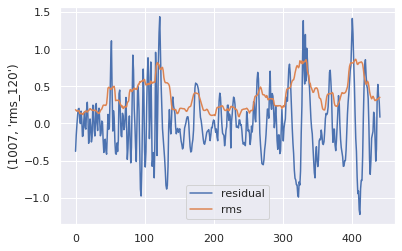
\includegraphics[scale=0.6]{residual_rms_example.png}
    \caption{An illustration of the relation between the high-frequency IBI signal (blue) and the RMSSD (orange). The RMSSD is calculated by taking the signal’s root mean square (RMS) on a moving time-window, for the high-frequency component.}
    \label{fig:rms_example}
\end{figure}

Third, we will elaborate the quantitative analysis of the drumming coordination. We will apply \emph{discrete relative phase analysis} \citep{abp2017symmetry} between pairs of drumming signals, followed by entropy calculation on the resulting distribution, to extract an index for beat-to-beat drumming coordination. We will also look at correlations in beat pacing during the session. These constitute enhancements to the single coordination index in the previous work.

Fourth, we will embed the heart-rate IBI signals of each triad in a 2D metric space in order to visualize and characterize synchrony within each group. Representing each signal as a point and positioning it relative to the other points in 2D according to the pairwise \emph{angular distances}, the triangular shape formed by the three points constitutes a concise  visual representation of each triad's interrelations. This triangle is also expedient in giving an intuitive interpretation to both first- and second-order statistics of the group's synchrony. We intend to demonstrate that the second-order statistic is essential to explaining the psychological target variables, namely the group cohesion and drumming coordination. Figure~\ref{fig:triangles} shows initial results with several different sizes and shapes of triangles apparent. 


\begin{figure}[h]
    \centering
    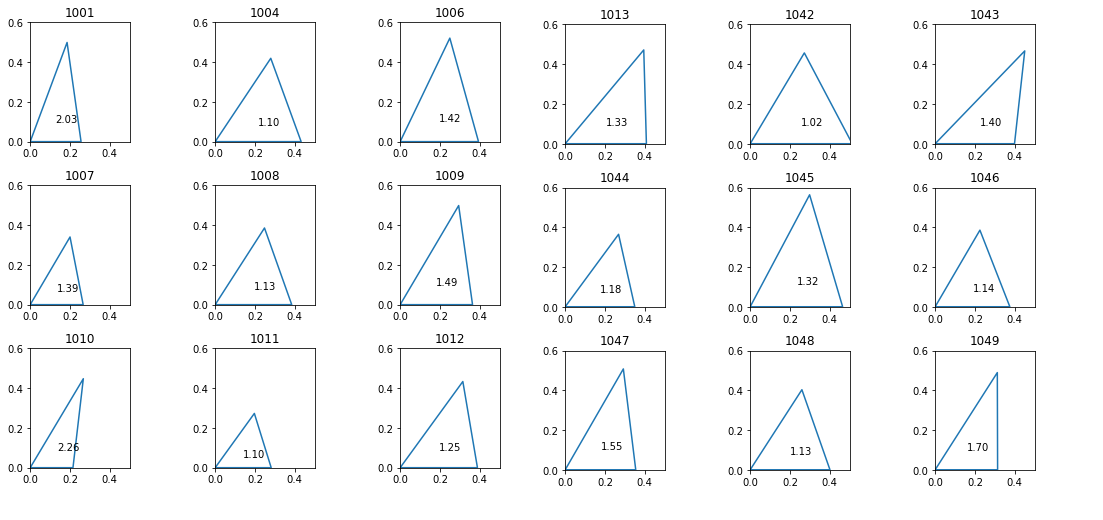
\includegraphics[scale=0.35]{triangles_coupling_modes_landscape.png}
    \caption{Characterizing physiological interactions between groups consisting of 3 participants. Plots of the triangles formed by calculating the angular distance of cardiac IBI interactions for each triad's interaction session. The title of each plot indicates the group number. The number appearing inside each triangle is the \emph{form-factor}, the ratio of the average of the two longer sides to the shortest side of the triangle.} 
    \label{fig:triangles}
\end{figure}

Finally, with the richer and more nuanced descriptions of both the heart-rate synchrony and the drumming coordination, we plan to uncover meaningful quantitative relationships between the physiological and the sensorimotor aspects of the interaction, and establish additional links between the different variables.  

\section{Preliminary results on the characterization of triads using angular distance}

For each session, we will calculate the angular distances between the three IBI signals. Taking the three distances as the three sides of a triangle, then ordering the sides from short to long counterclockwise and allowing the shortest side to rest on the x-axis, we will obtain images as depicted in 
Figure~\ref{fig:triangles}.

We then extract for each  triangle, the ratio of (the average of) the two longer sides to the shortest edge. This ratio characterizes the triangle's \enquote{form factor}. Plotting the length of the shortest side on the x-axis and the form-factor on the y-axis, we arrive at the chart depicted in Figure~\ref{fig:formfactor}A. In Figure~\ref{fig:formfactor}B, We have used four labels to tag the different triangles and define four groups with different characteristics of interaction:
\begin{enumerate}
    \item \emph{Two-way coupling} - these are the triangles with a short edge and a high form-factor.
    \item \emph{No coupling} - these are the triangles with three long edges.
    \item \emph{Three-way coupling} - these are triangle with three short edges.
    \item \emph{Transition} - The transition area is characterized by the two measures assuming values close to the population's median.
\end{enumerate}
We propose to use a support vector machine (SVM) to find the optimal separating hyperplanes among the four groups. We then wish to use this division of the space and the associated parameters in order to examine triadic relations in other experiments, and to probe whether other characteristics of the same groups of triads, such as drumming synchrony and group cohesion, are notably different when comparing the four populations of triads.   



\begin{figure}
    \centering
    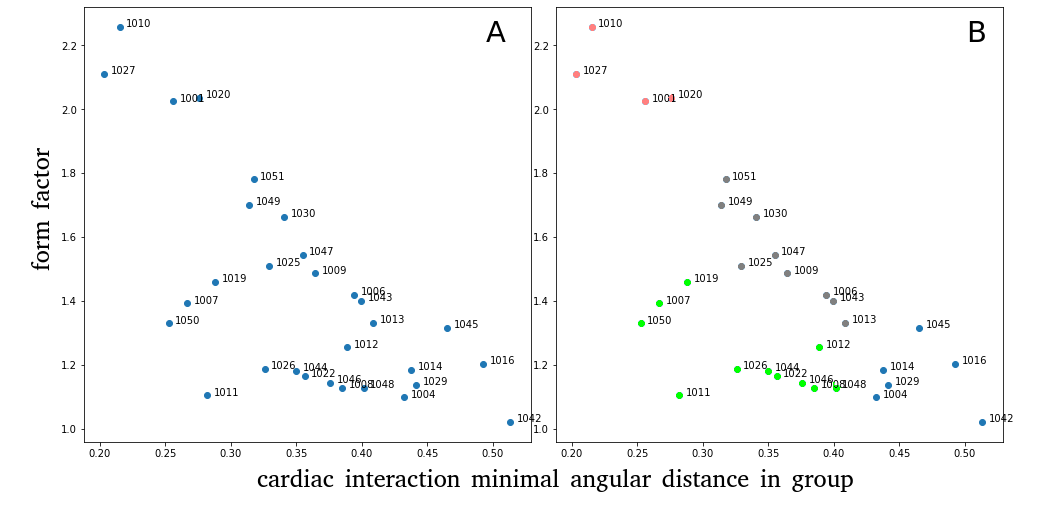
\includegraphics[scale=0.35]{coupling_clusters_and_original_sbs.png}
    \caption{Characterization of cardiac interactions in triads using the triangle's shorter edge and the form-factor. A: The xy-coordinate of the point corresponding to each triad is based on the length of the shorter edge (x axis) and its form factor (y axis). B: Four clusters (distinguished by the dot colors) with different interaction characteristics can be identified }
    \label{fig:formfactor}
\end{figure}

\section{Contributions based on methods from computer science}
We'd like to point to the original contributions that will involve methods developed in the domains of computer science and statistical machine learning.

The mathematical notion of a distance metric is often applied in machine learning in order to find similar samples and to embed a high-dimensional data point in a low-dimensional space. Here, it will help in summarizing the relationships among the three signals.

Shannon entropy will be employed in order to derive a distance measure from the drumming's relative phase charts and to quantify drumming synchronization.

Finally, our research involves characterizing relationships and finding interesting connections among several variables: synchrony indices in different bands and during different sessions; drumming performance indices in two separate drumming sessions; psychological traits and reactions to the group interaction. This is essentially a task of knowledge discovery in databases (KDD), where a large array of supervised and unsupervised machine learning methods may be applied. The choice of methods and models  will have to account for the number of records at our disposal. Some methods that we consider apt, are classification and regression trees (CART), clustering analysis, and latent-variable modeling using the expectation-maximization (EM) algorithm.




\vspace{1cm}



\appendix
\chapter{Experimental Details}
\section{Technical background on the IBI signal}
The physiological signal to be analyzed in the current work is the IBI signal. The IBI signal is derived from the ECG (electric potential between electrodes placed on the subject's torso) as follows: The timing of the \emph{R-peak} (see Figure \ref{fig:qrs}) of each heartbeat is detected. The time differences between successive peaks are known as RR-intervals, and are measured to within 2 milliseconds. The RR-intervals are then interpolated and resampled on a regular time interval of 500 milliseconds. 
Both the \enquote{raw} RR-intervals and the interpolated signals are provided as output from the experimental hardware and accompanying software suite.

\begin{figure}
    \centering
    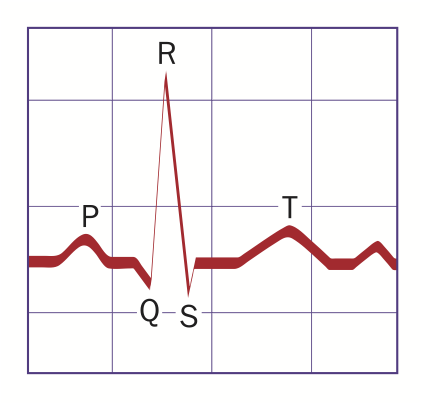
\includegraphics[scale=0.3]{normalqrs_simplelabels.png}
    \caption{Illustration of an ECG waveform, with labels for each peak. The prominence of the R peak is apparent. Source: \cite{HealioQRSChart}}
    \label{fig:qrs}
\end{figure}

\section{Experiment itinerary and details of data recorded}
A brief description of the experiment on which this work focuses follows. The experiment as described below was repeated 50 times, with different teams of three members each. For more details, see \cite{gordon2020physio}.
\begin{itemize}
    \item Before arriving, each participant had to fill in and submit a personality questionnaire which focuses on social affinity.
    \item Just before the interaction started, the participants filled another questionnaire, regarding their current mood, sleep, and caffeine intake.

    \item Each team's interaction was subdivided into 4 sessions. The sessions were recorded (video, audio), and electrodes were used to collect continuous ECG readings from the participants. 
    \begin{itemize}
        \item In the first session, team members were simply asked to relax. This is the first of two \emph{baseline} sessions.
        \item In the second session, team members were instructed to follow a pre-recorded drumming tempo. Each participant played on his or her own electronic drum pad, allowing us to record the beats of each player. This session lasted 4 minutes. Half the teams were randomly selected for one type of tempo, and the other half followed a different tempo.
        \item At this point, the participants filled in their responses to questions regarding both perceived drumming synchrony, and affect.
        \item Next, each team played the drums again, this time without any background tempo (\emph{freestyle} session).
        \item Following the freestyle sessions, an additional round of questions regarding affect was administered. 
        \item In the final session, the team members again were in the same room without performing any task. This is the second baseline session.
    \end{itemize}
\end{itemize}
Note: Participants were pre-screened for musical  background. Respondents with significant musical experience were not admitted.




\bibliography{ref}
\end{document}

